%% %%%%%%%%%%%%%%%%%%%%%%%%%%%%%%%%%%%%%%%%%%%%%%%%%
%% Template for a conference paper, prepared for the
%% Food and Resource Economics Department - IFAS
%% UNIVERSITY OF FLORIDA
%% %%%%%%%%%%%%%%%%%%%%%%%%%%%%%%%%%%%%%%%%%%%%%%%%%
%% Version 1.0 // November 2019
%% %%%%%%%%%%%%%%%%%%%%%%%%%%%%%%%%%%%%%%%%%%%%%%%%%
%% Ariel Soto-Caro
%%  - asotocaro@ufl.edu
%%  - arielsotocaro@gmail.com
%% %%%%%%%%%%%%%%%%%%%%%%%%%%%%%%%%%%%%%%%%%%%%%%%%%
\documentclass[11pt]{article}
\usepackage{UF_FRED_paper_style}
\usepackage{tabularx}
\usepackage{siunitx}
\usepackage{tipa}
\usepackage{textcmds}
\usepackage{multirow} 
%\usepackage{xcolor}
\usepackage[dvipsnames]{xcolor}
\usepackage{soul}
\definecolor{HLColor}{RGB}{230,230,250}
\sethlcolor{HLColor}
\usepackage[
    backend=biber,
    style=numeric,
  ]{biblatex}

\addbibresource{references.bib}
%% ===============================================
%% Setting the line spacing (3 options: only pick one)
%\doublespacing
% \singlespacing
\onehalfspacing
%% ===============================================
 
%\setlength{\droptitle}{-5em} %% Don't touch

% %%%%%%%%%%%%%%%%%%%%%%%%%%%%%%%%%%%%%%%%%%%%%%%%%%%%%%%%%%
% SET THE TITLE
% %%%%%%%%%%%%%%%%%%%%%%%%%%%%%%%%%%%%%%%%%%%%%%%%%%%%%%%%%%

% TITLE:
\title{\textbf{User Interface Design: Deliverable D4}\\Moodtracker for Companies}

% AUTHORS:
\author{Laurenz Kottek\\ Céline Nöhl\\ Alexandros Tsaparas\\ Noé Barbera}


    
% DATE:
\date{\today}

% %%%%%%%%%%%%%%%%%%%%%%%%%%%%%%%%%%%%%%%%%%%%%%%%%%%%%%%%%%
% %%%%%%%%%%%%%%%%%%%%%%%%%%%%%%%%%%%%%%%%%%%%%%%%%%%%%%%%%%
\begin{document}
% %%%%%%%%%%%%%%%%%%%%%%%%%%%%%%%%%%%%%%%%%%%%%%%%%%%%%%%%%%
% %%%%%%%%%%%%%%%%%%%%%%%%%%%%%%%%%%%%%%%%%%%%%%%%%%%%%%%%%%
% ABSTRACT
% %%%%%%%%%%%%%%%%%%%%%%%%%%%%%%%%%%%%%%%%%%%%%%%%%%%%%%%%%%
% %%%%%%%%%%%%%%%%%%%%%%%%%%%%%%%%%%%%%%%%%%%%%%%%%%%%%%%%%%
{\setstretch{.8}}
\maketitle 

\vspace{15mm}


\tableofcontents
\newpage

\section{Introduction}
The following sections contain a description of the structure and functionality of our prototype. In addition, the associated state transition network is presented and the usability tests are described. Functional requirements with their priority and important design ideas are then presented. As we are still only looking at the team leader side in this report and are leaving out the user interface of the team members due to the scope of work, we have finally looked at how the app can be developed further. Here we focus in particular on the interface of the team member side.
\clearpage

\section{State-Transisition Network}

\begin{figure}[h!]
    \centering
    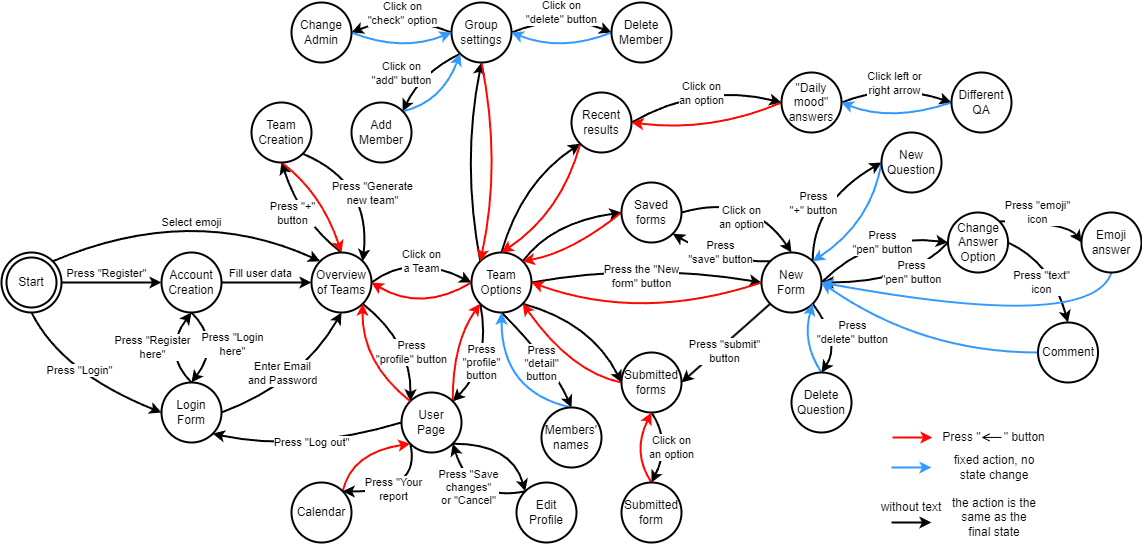
\includegraphics[width=1.4\textwidth, angle = 90]{figures/State-Transition Network.drawio.png}
    \caption{State Transition Network for the Mood Tracker App}
    \label{fig:STN}
\end{figure}

\clearpage

\section{Prototype}
The prototype was developed as a smartphone application. Several functions extended the LoFi prototype from D3 for this release. In addition, some adjustments were made according to the results of the user tests. The changes and enhancements include a feedback screen that provides feedback on whether the creation of a team or a new form was successful, as well as the replacement of some icons for a better understanding of the function. The option to create a new user profile or change the registered profile has also been added. Finally, profile settings have been added. The final prototype can be found under this \href{https://www.figma.com/proto/eesoN637wOm4ooDvH1GrsL/Mood-Tracker?type=design&node-id=33-360&t=20IVLZwIw9F8b4pc-1&scaling=min-zoom&page-id=0%3A1&starting-point-node-id=33%3A360&mode=design}{\textbf{Link}} and is attached as a Figma file.\\
In \autoref{fig:startscreen} you can see the start screen. From here you can either create a new profile, change the logged-in profile, or answer the day's question to get to the team overview. If you want to create a new profile, you will be taken to the screen shown in \autoref{fig:register}. If you want to change the registered profile, you will be taken to the screen shown in \autoref{fig:login}.
\begin{figure}[h!]
     \centering
     \begin{subfigure}[b]{0.3\textwidth}
         \centering
         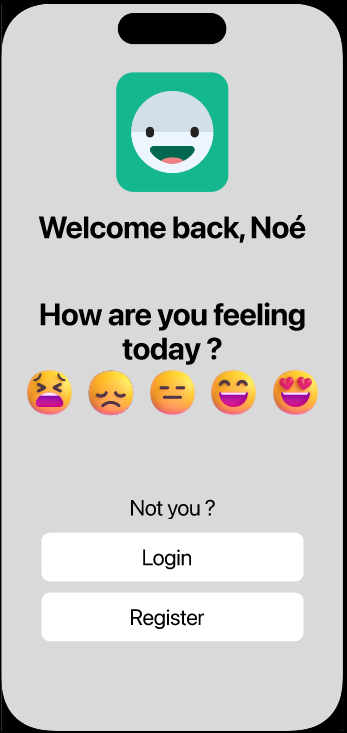
\includegraphics[width=\textwidth]{figures/start screen.PNG}
         \caption{Start screen. \\ \mbox{}}
         \label{fig:startscreen}
     \end{subfigure}
     \hfill
     \begin{subfigure}[b]{0.3\textwidth}
         \centering
         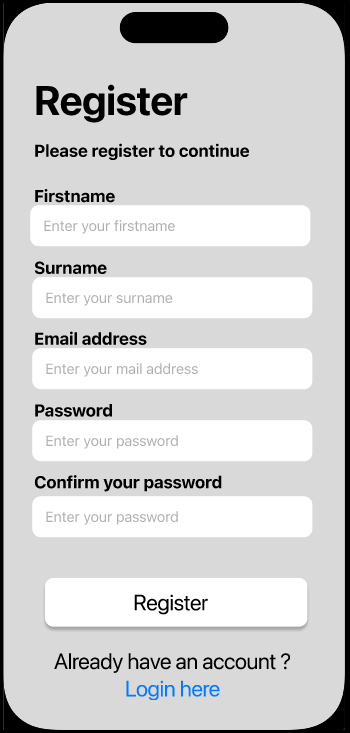
\includegraphics[width=\textwidth]{figures/register.PNG}
         \caption{Screen to register.\\ \mbox{}}
         \label{fig:register}
     \end{subfigure}
          \hfill
     \begin{subfigure}[b]{0.3\textwidth}
         \centering
         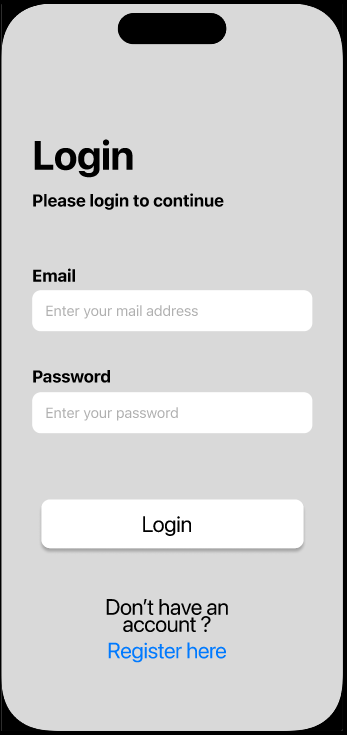
\includegraphics[width=\textwidth]{figures/login.PNG}
         \caption{Screen to log in to an\\ existing profile.}
         \label{fig:login}
     \end{subfigure}
        \caption{Start screen, login screen and register screen of the Moodtracker app.}
\end{figure}

Once the login is complete, the user is taken to the team overview, which is shown in \autoref{fig:teamoverview}. Here users can access their profile, create a new team or access an individual team.  If a new team is to be created, the screen shown in \autoref{fig:newTeam} is displayed. The overview of a single team can be seen in \autoref{fig:individualTeam}.
\begin{figure}[h!]
     \centering
     \begin{subfigure}[b]{0.3\textwidth}
         \centering
         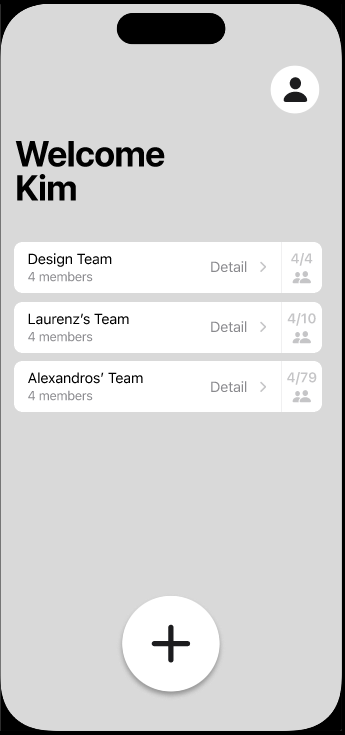
\includegraphics[width=\textwidth]{figures/team overview.PNG}
         \caption{Screen with the team overview. }
         \label{fig:teamoverview}
     \end{subfigure}
     \hfill
     \begin{subfigure}[b]{0.3\textwidth}
         \centering
         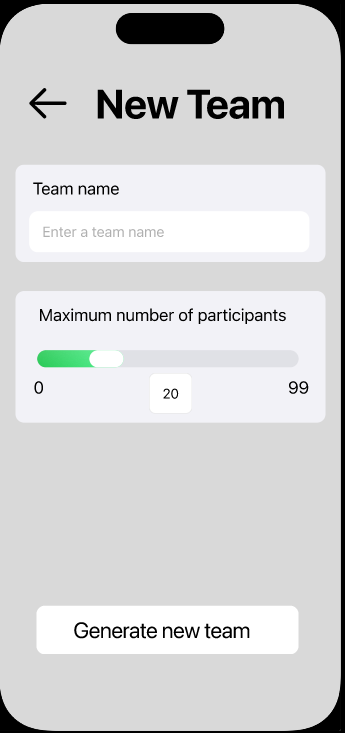
\includegraphics[width=\textwidth]{figures/new team.PNG}
         \caption{Screen to create a new team.}
         \label{fig:newTeam}
     \end{subfigure}
          \hfill
     \begin{subfigure}[b]{0.3\textwidth}
         \centering
         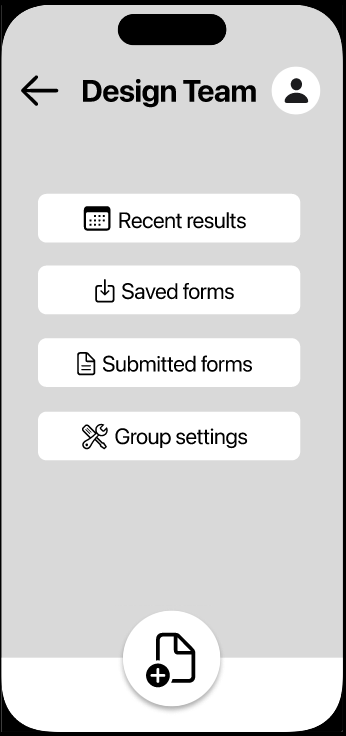
\includegraphics[width=\textwidth]{figures/team.PNG}
         \caption{Overview of one individual team.}
         \label{fig:individualTeam}
     \end{subfigure}
        \caption{Team overview, creating a new team and the individual team overview.}
\end{figure}
From the profile overview shown in \autoref{fig:profile}, you can either access the daily moods report, which can be seen in \autoref{fig:report}, or make settings for the profile. 

\begin{figure}[h!]
     \centering
     \begin{subfigure}[b]{0.3\textwidth}
         \centering
         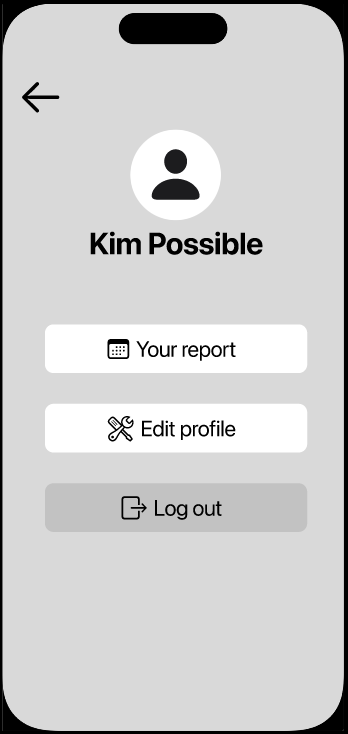
\includegraphics[width=\textwidth]{figures/profile overview.PNG}
         \caption{The user's profile.\\ \mbox{} }
         \label{fig:profile}
     \end{subfigure}
        \hspace{1cm}
     \begin{subfigure}[b]{0.3\textwidth}
         \centering
         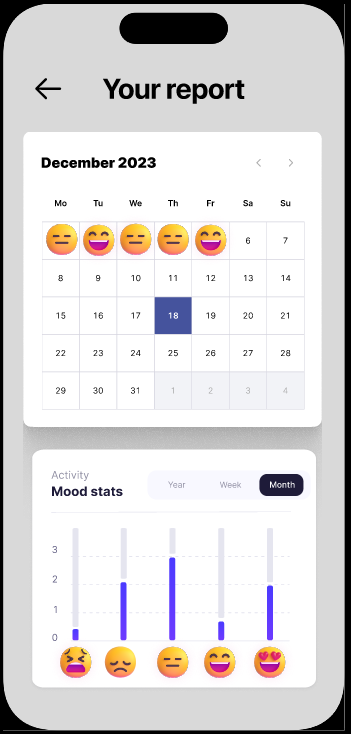
\includegraphics[width=\textwidth]{figures/report.PNG}
         \caption{Report of the recent daily mood questions.}
         \label{fig:report}
     \end{subfigure}
        \caption{Profile overview and report of daily mood questions.}
\end{figure}


\clearpage

\section{User Tests}
The following describes the goals of our User Tests, how we selected the participants for
the tests, performed the user tests, and finally analysed them

\subsection{Goals of the User Tests}
Our current prototype's user test aims to pinpoint areas needing improvement and assess the success of our changes from previous tests. As this is our project's final testing phase, we are ensuring all implemented features work seamlessly and are easily understandable, promoting user satisfaction. \\
We have expanded our user test task description to include more tasks and detailed descriptions, aiding in pinpointing challenging tasks and those functioning well. \\
As for the previous user tests, we will circulate a brief survey to gather participant feedback on ease, difficulty, likes, and dislikes. In that way, we can figure out what we need to work on and what is already good.\\
Our new user tests will focus on specific tasks. Some of the tasks were previously tested, while others are new or untested:

\begin{enumerate}

    \item Functions previously tested:
    \begin{itemize}
        \item Team creation
        \item Form creation
        \item Submitting and saving forms
    \end{itemize}

    \item Functions not yet tested: 
    \begin{itemize}
        \item Account creation
        \item Editing questions in form creation
        \item Navigation within "saved" and "submitted" forms
        \item Profile editing
        \item Navigation through "report"
        \item Navigation in "recent results"
        \item Logging out of accounts
    \end{itemize}
    
\end{enumerate}

\subsection{Participants}
Our app is basically aimed at companies, but as this app is being developed as part of a university course, it is unfortunately not possible for us to carry out user tests with users from the right target group. Therefore, at the beginning of the test, we asked users to put themselves in the role of a team leader in a company. We also tried to keep the group as diverse as possible, but this proved difficult due to our almost exclusively student environment. 

\subsection{Execution and Setup}
The procedure for the user tests was largely the same as for the previous tests in D3. First, the test subjects were given a task description describing the scenario and some problems with Figma and how to solve them. Here, the filling in of free text fields is discussed in particular, as Figma does not offer any option for this. We solved the problem with a predefined text.\\
The tasks to be performed with the app are then presented. The task sheet is attached to the report as a pdf file under the name "Task Description". If the participant has no further questions, the test can begin. Due to the space available, the participant and a member of our group (supervisor) sit next to each other, as shown in \autoref{fig:UserTestScheme}.\\
\begin{figure}[h!]
    \centering
    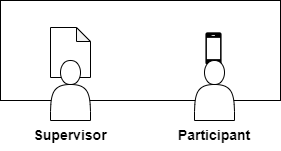
\includegraphics[width=0.5\textwidth]{figures/UserTest_Scheme.png}
    \caption{Scheme of the setup for the user tests.}
    \label{fig:UserTestScheme}
\end{figure}

The supervisor takes notes during the test. The participants use the prototype on a smartphone. After the tasks are completed, the participants fill out a survey about the interface and the app in general. The survey is also attached to this report. \autoref{fig:execution} shows a picture taken during one user test.
\begin{figure}[h!]
    \centering
    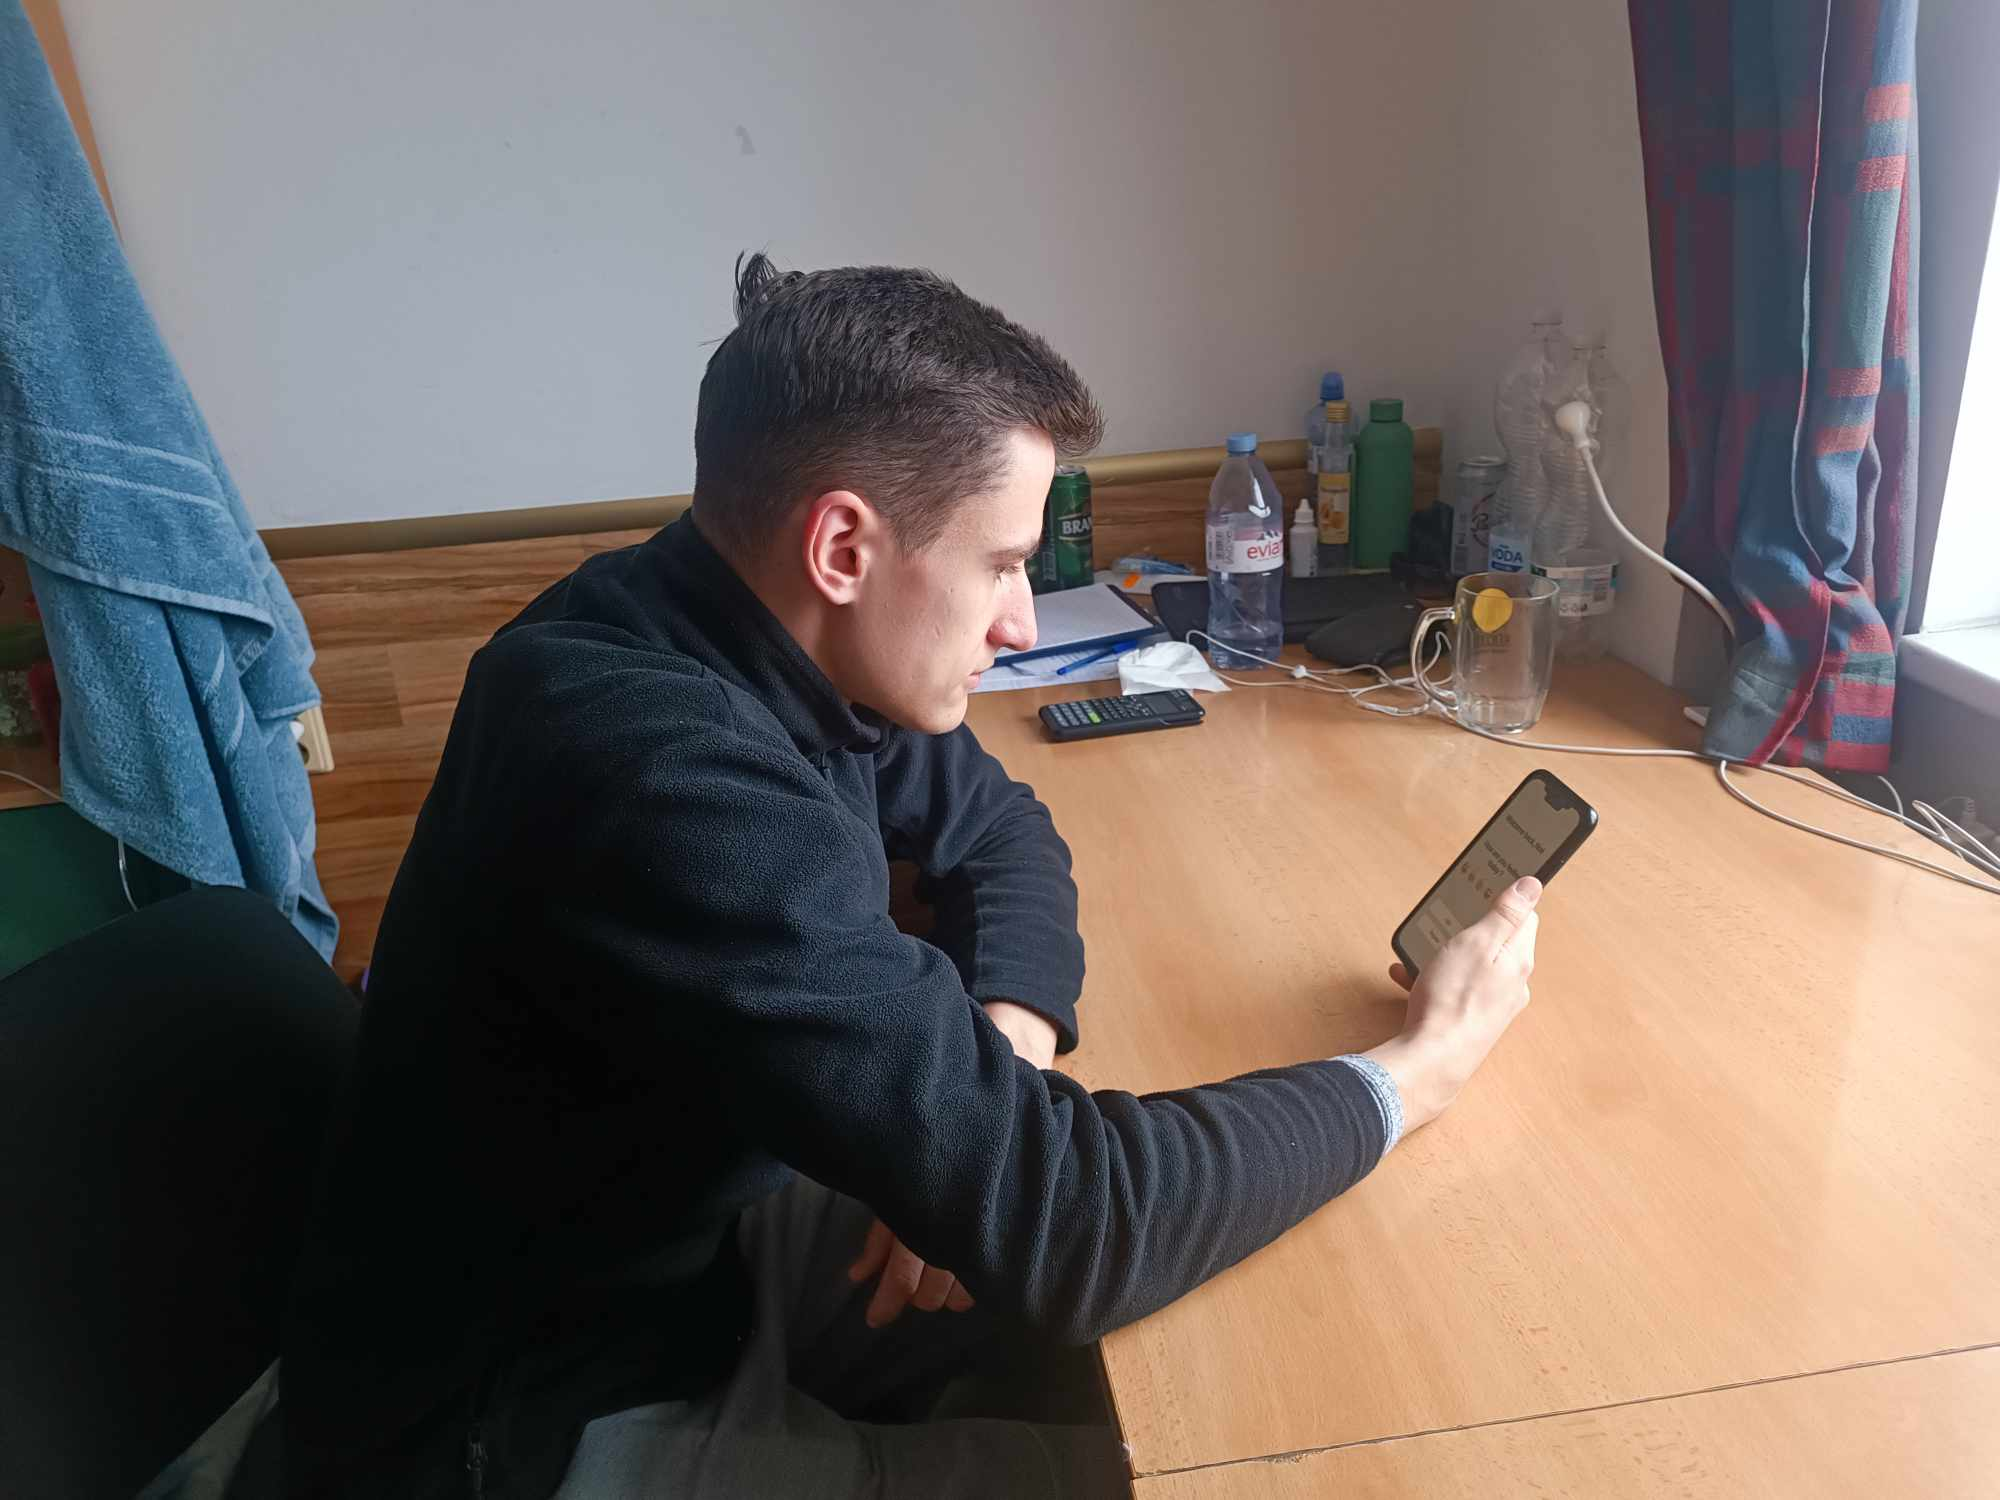
\includegraphics[width = 0.6\textwidth]{figures/Kostas_2.png}
    \caption{One participant during the user test.}
    \label{fig:execution}
\end{figure}




\subsection{Evaluation}
Before we started planning the user tests, we thought about what exactly the goal was and which aspects we wanted to test. To obtain comparable results, the survey was structured in the same way as the survey from D3. The survey was based on the tasks that the test subjects had to complete so that we could obtain precise feedback. The survey can be viewed at this \href{https://docs.google.com/forms/d/1XZn5U9J93oJQlkRKYR0nUfQ5ODQfRJeZ9GHHDy1MJC8/edit}{\textbf{Link}} or as a pdf file. The results are also attached as a pdf file. The survey was divided into the following sections: general feedback, task-specific feedback and likeability and improvement. In addition, the survey contained some open questions where participants could add their remarks and comments that were not covered by the other questions.

\subsection{Results}
10 Participants took part in our user test. Of course, this is not a statistically relevant number, but it can still give us some initial feedback on our app. \\
After the participants had completed the user tests, we collected some information about their experience with the user interface. Below are the results of the survey for some of the questions. The survey was carried out using Google Forms, which is why it is not possible to show only an absolute number without a percentage in the results. We are of course aware that the percentages are not meaningful with this small sample size. The detailed results of the survey can be accessed via the \href{https://docs.google.com/forms/d/1XZn5U9J93oJQlkRKYR0nUfQ5ODQfRJeZ9GHHDy1MJC8/viewanalytics}{\textbf{Link}} and are attached as a pdf file. As can be seen in \autoref{fig:question1}, users were consistently satisfied with the app.
\begin{figure}[h!]
    \centering
    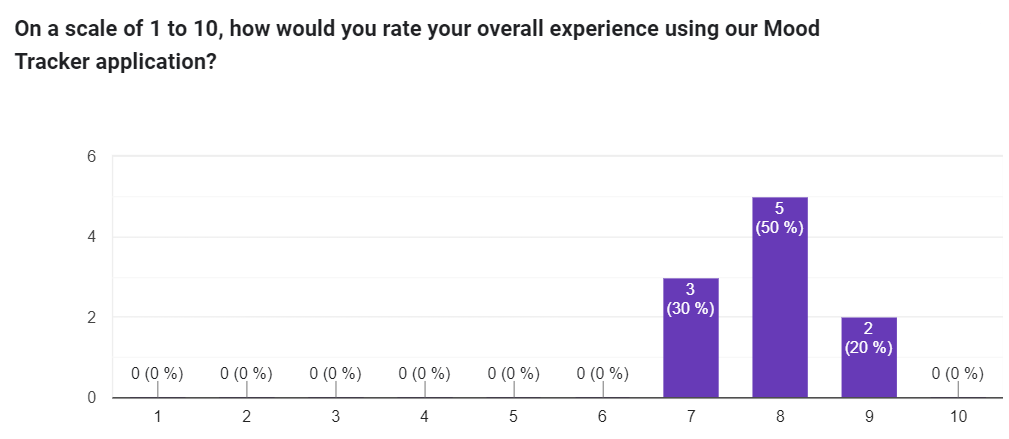
\includegraphics[width = \textwidth]{figures/Question 1.PNG}
    \caption{Caption}
    \label{fig:question1}
\end{figure}
\clearpage 
The users were also asked whether they had any problems while carrying out the tasks. The result of this question can be seen in \autoref{fig:question2}. 
\begin{figure}[h!]
    \centering
    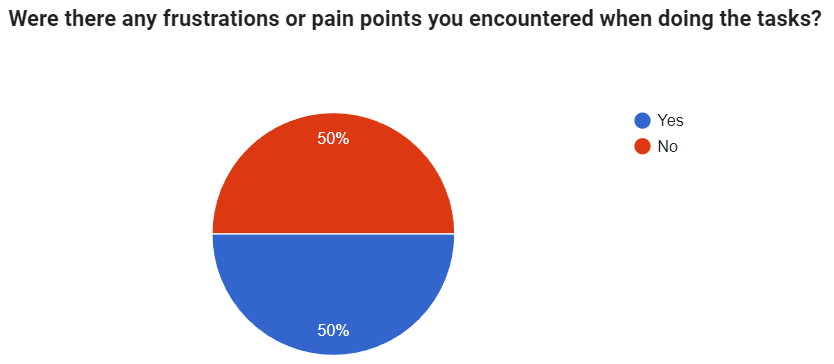
\includegraphics[width = \textwidth]{figures/Question 3.PNG}
    \caption{Caption}
    \label{fig:question2}
\end{figure}

The next question in \autoref{fig:question3} was asked to find out exactly which problems occurred and why they occurred in the first place. Various design decisions, such as the blurred emojis or the overview of the survey results, were cited as reasons. Other reasons were attributed to the technical capabilities of Figma or the basic structure of the prototype. 
\begin{figure}[h!]
    \centering
    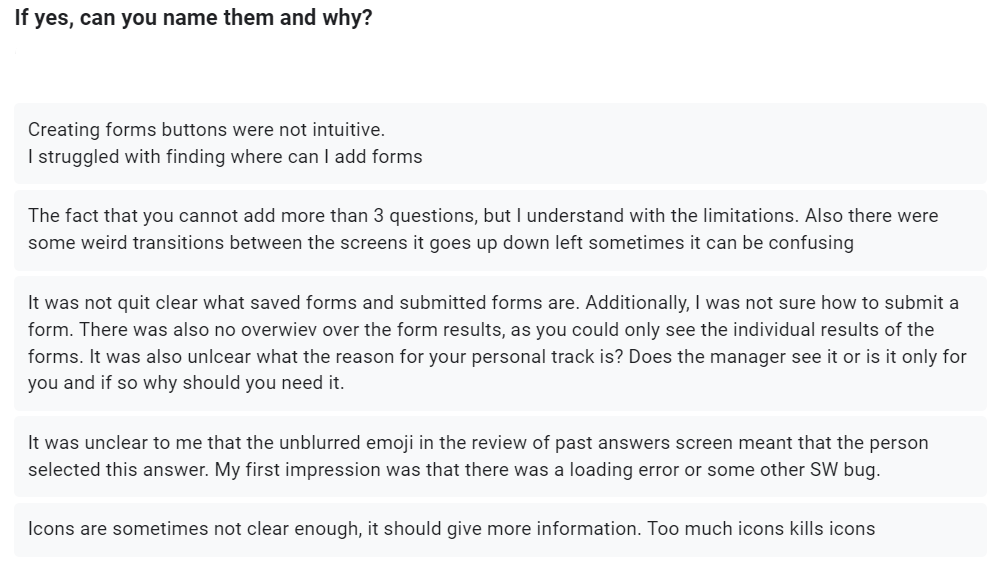
\includegraphics[width = \textwidth]{figures/Question 4.PNG}
    \caption{Caption}
    \label{fig:question3}
\end{figure}
\clearpage
One of the last questions, as seen in \autoref{fig:question4}, was then aimed at requests for improvement and other suggestions. Here, design ideas such as the choice of colors or the number of emojis were mentioned. Other points were again related to the prototype. Here, the main problem was again the text input, which is difficult to manage with Figma.
\begin{figure}[h!]
    \centering
    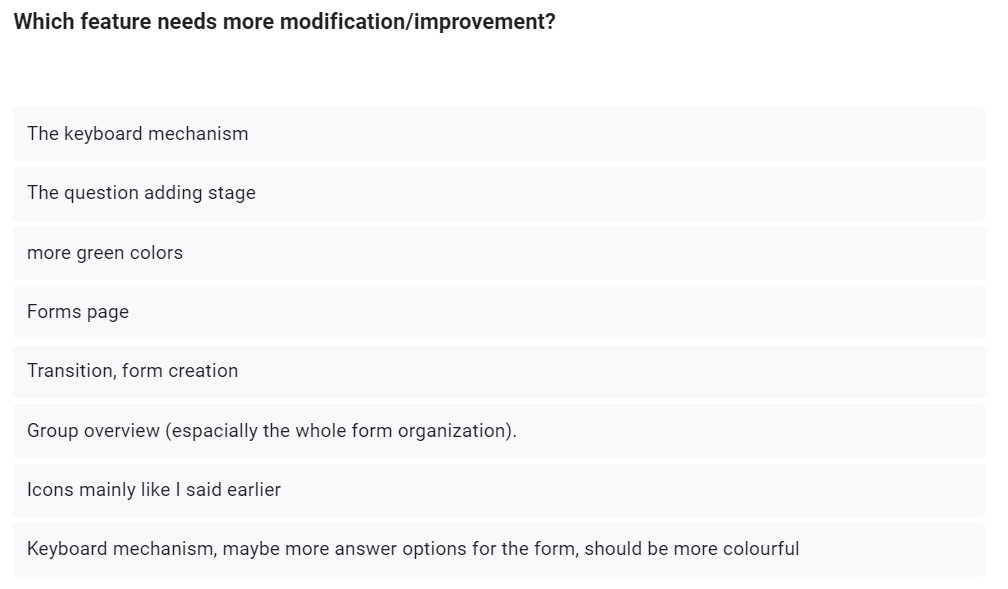
\includegraphics[width = \textwidth]{figures/Question 5.PNG}
    \caption{Caption}
    \label{fig:question4}
\end{figure}

\paragraph{Conclusion}\mbox{}\\
In conclusion, we can say that the users liked our app, but there are still some points that need improvement. The most popular feature of our app was the personal report, i.e. the tracking of personal mood independently of the forms. The minimalistic and clear design of our app was also perceived as pleasant, although one user suggested using more green color accents. One point of criticism that was repeatedly raised was the text input. However, this is negligible as it is not the implementation of the prototype that is responsible for this, but Figma. Another point of criticism was the creation of the forms. The test subjects found it difficult to add an additional question or change the question option. This is a point that should obviously be improved. 
In summary, however, the feedback was positive with only a few points that really need improvement.



\clearpage
\section{Documentation for Developers}
The developer documentation focuses on fundamental (web)app features, refining user experience, and specific design elements.
We aim to ensure the app is user-friendly, meets modern standards, and delights users with its design. We structured the documentation from most to least crucial functionalities.

\subsection{Functional Requirements}
    \paragraph{1. General application functionality} \mbox{} \\
    Our primary objective is to develop both a web and mobile app that operates fluently, with a focus on the mobile version as the app is meant for regular use. Priority one is ensuring smooth operation on Android and iOS devices with touch-based navigation.

    \paragraph{2. High Priority features:} \mbox{} \\
    Initially, our focus was on implementing profile creation and login features. Following this, we will integrate a daily mood tracking feature, allowing users to select an emoji daily to save their daily mood. This forms the basis for our mood tracker app. Once established, we'll proceed to develop team creation functionalities, enabling users to create and join teams.
    
    \paragraph{3. Medium Priority features:} \mbox{} \\
    Once the foundational elements are set, our development efforts will shift to enhancing app usability. We are looking to enable users to create forms, edit questions, and send these forms to specific team members. We'll also expand team settings to facilitate additions, access rights, or removals. Additionally, a mood overview must be integrated into the app while tracking mood.
    
    \paragraph{4. Least Priority Features:} \mbox{} \\
    With the foundational work complete, we'll focus on further feature additions for better usability. This includes diversifying form creation to accommodate various question types and response formats. Additionally, the mood overview could include monthly reports and statistical insights on mood fluctuations.
    


\subsection{Design Ideas}
While planning our user interface and working on the mood tracker idea, we aimed for a simple and easy-to-use design. An easy navigation within the app was our main goal. Although we did not have that many functions already, it turned out to be not as easy as we thought.\\
In order to reach the mentioned goals, we have kept the design simple, with a light grey background, black font for clarity, and highlighted white buttons for better contrast. \\
For intuitive navigation, the landing screen consistently displays team overviews. Within teams, prominent buttons facilitate easy navigation to various sections. Uniform symbols and their placement ensure consistency, such as the top-left corner always leading back to the previous page (finally leading to the team overview).\\
Aiming for easy and fast navigation, the mood overview is only two clicks away from the landing screen and is accessed through the profile button. 


\section{Ideas for the Future}
While our focus was primarily on the team leader part of the application, we did not think about certain features essential for regular team members. Despite the prototype encompassing several necessary features for team members, such as login, mood calendar, and profile management, there's still work to be done. Additionally, although we've addressed many functional aspects, there's ample room for future enhancements and improvements across various functionalities and use cases. Therefore, we decided to spotlight additional ideas we have, in the following abstract.

\paragraph{1. Prioritizing the team member aspect:}\mbox{} \\ 
Enabling communication between team leaders and members remains a key goal. We must introduce features for team members to receive prepared forms, fill them out, and subsequently save or submit them. To maintain consistency and user-friendliness, we aim to design and implement these functionalities similar to form creation. This approach ensures users can seamlessly transition between roles as team leaders and team members across different teams.

\paragraph{2. Expansion of well-being features:}\mbox{} \\ 
Currently, our approach's well-being features revolve around personal daily mood tracking and forms. We envisage augmenting these features to further enhance user well-being. Enhancements include broadening daily mood tracking to enable users to provide detailed daily feedback beyond a single summarizing emoji. Automatic daily or weekly questions post-login could be integrated for users to respond to.\\
Moreover, the app can generate monthly summaries of daily moods, especially beneficial when users provide detailed feedback. This enables users to acquire a more accurate overview of mood fluctuations and potentially receive recommendations for change. As user numbers increase, we're considering incorporating a long-term chat function with human psychological support, as AI-chat bots, while improving, may not match human interaction in this context.


\paragraph{3. Target Group Survey:}\mbox{} \\ 
Although we conducted preliminary research on potential use cases in D1, a more in-depth study is imperative for a project of this nature. Specifically, we need to engage potential customers, users, and companies in comprehensive user and use case research. By eliciting their needs, thoughts, and current challenges, we aim to make the project more human-centered (UCD). This approach ensures a more user-centric development process.

% --------------------
\printbibliography

% ==========================
% ==========================
% ==========================


\end{document}